\section{Zielsetzung}
\label{sec:Zielsetzung}
Ziel dieses Versuch ist es die Elementarladung mithilfe des Millikan-Öltröpfchenversuchs zu bestimmen.
\section{Theorie}
\label{sec:Theorie}
Bei dem Millikan-Öltröpfchenversuch werden Öltröpfchen durchs Zerstäuben in das vertikale
elektrische Feld eines Plattenkondensators gebracht. Die Tröpfchen werden aufgrund der Reibung
elektrisch geladen, wobei diese Ladung ein ganzzahliges Vielfaches der Elementarladung ist.
Es wirkt die Gravitationskraft $\vec{F_g}=m \vec{g}$, die Reibungskraft 
$\vec{F_r} = - 6 \pi r \eta_L v_0$ und die elektrische Kraft $\vec{F_{el}} = q \vec{E}$.
Die Geschwindigkeit der Tröpfchen ist abhängig von den Richtungen der Kräfte, was in \autoref{fig:Abb_1} dargestellt wird.
\begin{figure}[H]
    \centering
    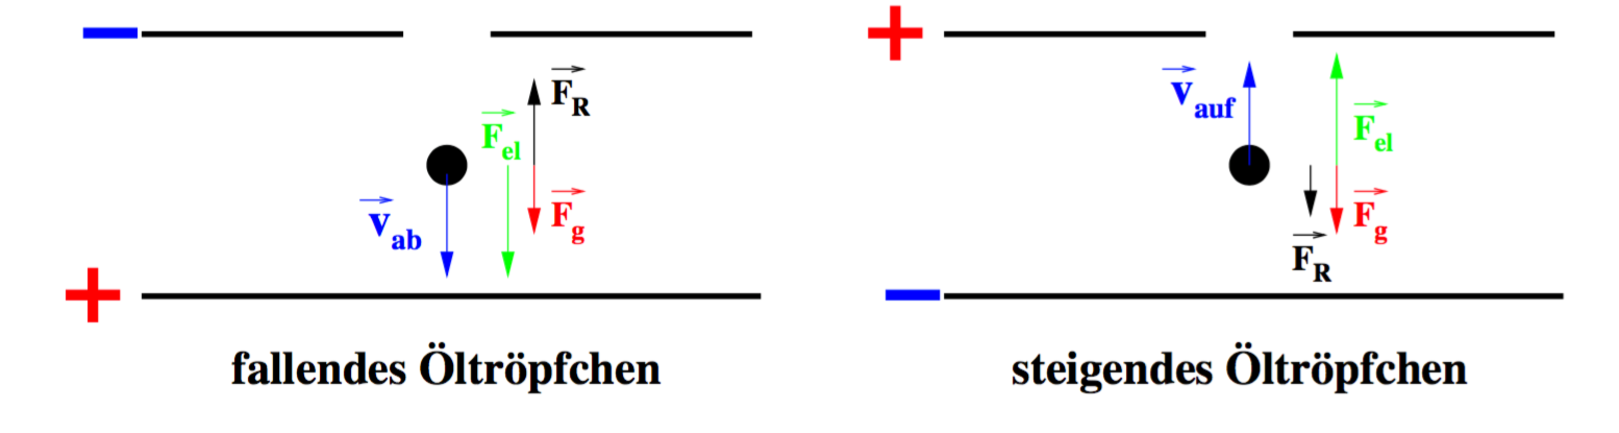
\includegraphics[width=0.7\textwidth]{Abbildungen/Abb_1.pdf}
    \caption {Schematische Darstellung der Kräfte in einem homogenen elektrischen Feld\cite[1]{V503}.}
    \label{fig:Abb_1}
\end{figure}
Liegt eine Spannung an der unteren Platte an, wirkt die elektrische Kraft in Richtung der Gravitationskraft.
Die Reibungskraft wirkt entgegen der beiden Kräfte und gegen die Geschwindigkeit $\vec{v_{ab}}$.
Es gilt die Kräftegleichung
\begin{equation}
    \frac{4 \pi}{3} r^3 (\rho_{Oel}-\rho_L)g - 6 \pi \eta_L r v_{ab} = - q E.
    \label{eqn:vab}
\end{equation}
Liegt eine Spannung an der oberen Platte an, wirkt die elektrische Kraft entgegen der Gravitationskraft.
Bei hinreichend hoher Feldstärke entsteht eine Aufwärtsbewegung, welche entgegen der Reibungskraft wirkt.
Es gilt die Kräftegleichung
\begin{equation}
    \frac{4\pi}{3} r^3 (\rho_{Oel}+\rho_L) g + 6 \pi \eta_L r v_{auf} = q E.
    \label{eqn:vauf}
\end{equation}
Durch die Auftriebskraft wird $m$ in der Gravitaionskraft korrigiert mit der reduzierten Dichte $\rho = \rho_{Oel}-\rho_L$.
Die Ladung kann mit \autoref{eqn:vab} und \autoref{eqn:vauf} zu
\begin{equation}
   q = 3 \pi \eta_L \sqrt{\frac{9}{4} \frac{\eta_L}{g} \frac{(v_{ab}-v{auf})}{(\rho_{Oel}-\rho_L)}} \frac{(v_{ab}+v{auf})}{E}
    \label{eqn:Ladung}
\end{equation}
bestimmt werden und der Radius zu
\begin{equation}
    r = \sqrt{\frac{9 \eta_L (v_{ab}-v{auf})}{2 g (\rho_{Oel}-\rho_L)}}.
    \label{eqn:Radius}
\end{equation}
Die Viskosität von Luft muss durch 
\begin{equation}
    \eta_{eff} = \eta_L \Biggl(\frac{r}{r + A}\Biggr) = \eta_L \Biggl(\frac{\rho r}{\rho r + B}\Biggr)
    \label{eqn:eta_kor}
\end{equation}
korrigiert werden, weil das Gesetz von Stokes nur gilt, wenn die Abmessung des Tröpfchens größer als die mittlere
freie Weglänge ist. Diese Korrektur wird auch als Cunningham-Korrektur bezeichnet, wobei $B = 6,17 \cdot 10^{-3}\,  Torr \cdot cm$ gilt.
Die Ladung wird mit 
\begin{equation}
    q^{\frac{2}{3}} = q^{\frac{2}{3}}_0 (1 + \frac{B}{(p r)})
    \label{eqn:Ladung_kor}
\end{equation}
korrigiert, wobei $p$ der Luftdruck ist.